\documentclass[aspectratio=169,11pt]{beamer}

\usepackage{plex-serif}
\renewcommand{\familydefault}{\rmdefault}
\usepackage[T1]{fontenc}
\usepackage{amsmath,amssymb,bm}
\usepackage{pifont}
\usepackage{tikz}
\usetikzlibrary{calc,positioning,shapes.geometric,shapes.symbols,arrows.meta,decorations.pathreplacing}
\graphicspath{{img/}}

% ---------- Palette ----------
\definecolor{navy}{HTML}{002B55}
\definecolor{steel}{HTML}{4D6FAD}
\definecolor{sky}{HTML}{5DADF5}
\definecolor{teal}{HTML}{3F8C8A}
\definecolor{slate}{HTML}{5B6475}
\definecolor{paper}{HTML}{FBFAF7}
\definecolor{ink}{HTML}{1C2233}
\colorlet{deepteal}{navy!55!teal}
\definecolor{amber}{HTML}{E0A526}

% ---------- TikZ overlay helpers ----------
\tikzset{
  invisible/.style={opacity=0,text opacity=0},
  visible on/.style={alt={#1{}{invisible}}},
  alt/.code args={<#1>#2#3}{\alt<#1>{\pgfkeysalso{#2}}{\pgfkeysalso{#3}}},
  focus on/.style={alt={#1{draw=teal,line width=1.3pt}{}}},
  emphasis on/.style={alt={#1{draw=deepteal,line width=1.3pt,fill=deepteal!4}{}}},
}

% ---------- Standard diagram styles ----------
\tikzset{
  >={Stealth[length=2mm]},
  arr/.style={->,line width=0.7pt,draw=slate},
  lbl/.style={font=\footnotesize,text=slate,align=center},
  block/.style={trapezium,trapezium stretches=true,minimum width=2.4cm,minimum height=1.55cm,
                line width=0.8pt,font=\bfseries},
  enc/.style={block,shape border rotate=270,fill=steel!12,draw=steel,text=navy},
  dec/.style={block,shape border rotate=90,fill=teal!10,draw=teal,text=teal!70!black},
  param/.style={rectangle,rounded corners=2pt,minimum width=0.95cm,minimum height=0.6cm,
                draw=steel,line width=0.8pt,fill=white,text=navy,font=\normalsize},
  op/.style={circle,draw=slate,line width=0.8pt,fill=white,inner sep=1pt},
  photo/.style={draw=slate!50,line width=0.5pt},
  chip/.style={rectangle,rounded corners=3pt,line width=0.8pt,inner xsep=7pt,inner ysep=4pt,
               font=\footnotesize,fill=white},
  neuron/.style={circle,minimum size=0.48cm,inner sep=0pt,line width=0.7pt,font=\scriptsize},
  mystery/.style={rectangle,rounded corners=5pt,draw=deepteal,line width=1.3pt,fill=white,text=deepteal,
                  font=\fontsize{24}{24}\fontseries{eb}\selectfont},
}

% ---------- Beamer theme ----------
\setbeamercolor{background canvas}{bg=paper}
\setbeamercolor{normal text}{fg=ink}
\setbeamercolor{alerted text}{fg=teal}
\setbeamercolor{structure}{fg=navy}
\setbeamercolor{block title}{bg=navy,fg=white}
\setbeamercolor{block body}{bg=slate!7,fg=ink}
\setbeamertemplate{navigation symbols}{}
\setbeamertemplate{blocks}[rounded][shadow=false]

\newcommand{\stripeTR}[3]{\fill[#3] (#1,9.2) -- ++(#2,0) -- ++(4.5,-3.15) -- ++(-#2,0) -- cycle;}
\newcommand{\stripeBL}[3]{\fill[#3] (#1,-0.2) -- ++(#2,0) -- ++(-4.5,3.15) -- ++(-#2,0) -- cycle;}

\setbeamertemplate{background}{%
  \begin{tikzpicture}[remember picture,overlay,shift={(current page.south west)}]
    \clip (0,0) rectangle (16,9);
  \end{tikzpicture}}

\setbeamertemplate{frametitle}{%
  \begin{tikzpicture}[remember picture,overlay,shift={(current page.north west)}]
    \fill[navy] (0,0) rectangle (16,-1.05);
    \node[anchor=west,text=white,font=\fontseries{eb}\selectfont\Large] at (0.72,-0.525)
      {\insertframetitle};
  \end{tikzpicture}
  \vspace*{0.78cm}}


 \setbeamertemplate{footline}{%
  \begin{tikzpicture}[remember picture,overlay,shift={(current page.south west)}]
    \node[anchor=west,font=\scriptsize,text=steel] at (0.72,0.32)
      {Variational Autoencoder \;\textcolor{slate!60}{|}\; CSE 200};
    \node[anchor=east,font=\scriptsize\bfseries,text=steel] at (15.3,0.32)
      {\insertframenumber/\inserttotalframenumber};
  \end{tikzpicture}}


 \setbeamertemplate{footline}{%
  \begin{tikzpicture}[remember picture,overlay,shift={(current page.south west)}]
    \node[anchor=west,font=\scriptsize,text=steel] at (0.72,0.32)
      {Variational Autoencoder \;\textcolor{slate!60}{|}\; CSE200};
    \node[anchor=east,font=\scriptsize\bfseries,text=steel] at (15.3,0.32)
      {\insertframenumber/\inserttotalframenumber};
  \end{tikzpicture}}

% ---------- Page canvas: draw in page coordinates (16 x 9 cm) ----------
% content zone ~ x 0.9..15.1, y 0.9..7.3
\newenvironment{canvas}
  {\begin{tikzpicture}[remember picture,overlay,shift={(current page.south west)}]}
  {\end{tikzpicture}}

% ---------- Reusable drawings ----------
% digit "image" thumbnail:  \thumb[opts]{pos}{digit}
\newcommand{\thumb}[3][]{%
  \node[draw=slate!50,line width=0.5pt,fill=white,minimum size=0.52cm,inner sep=0pt,text=ink,
        font=\small\fontseries{eb}\selectfont,#1] at (#2) {#3};}

% latent-space clusters. #1 = cloud radius (0 = plain points), #2 = scale of cluster centres
\newcommand{\clusters}[2]{%
  \pgfmathsetseed{4242}%
  \foreach \cx/\cy/\sx/\sy/\rot/\col in {
      -2.35/ 1.55/0.34/0.20/ 20/navy,
      -0.25/ 1.85/0.20/0.40/-25/teal,
       2.20/ 1.20/0.40/0.22/ 40/steel,
      -2.05/-1.35/0.30/0.28/  0/slate,
       0.60/-0.45/0.26/0.36/ 60/teal!55!white,
       2.40/-1.65/0.44/0.19/-15/steel!55!white}{%
    \foreach \k in {1,...,22}{%
      \pgfmathsetmacro\rr{min(2.1,sqrt(-2*ln(max(rnd,0.005))))}%
      \pgfmathsetmacro\tt{360*rnd}%
      \pgfmathsetmacro\px{#2*\cx + cos(\rot)*\sx*\rr*cos(\tt) - sin(\rot)*\sy*\rr*sin(\tt)}%
      \pgfmathsetmacro\py{#2*\cy + sin(\rot)*\sx*\rr*cos(\tt) + cos(\rot)*\sy*\rr*sin(\tt)}%
      \ifdim #1pt>0pt \fill[\col,opacity={0.024/#1}] (\px,\py) circle (#1); \fi
      \fill[\col] (\px,\py) circle (0.055);
    }}}
% digit labels next to the clusters (#1 = centre scale)
\newcommand{\clusterlabels}[1]{%
  \foreach \cx/\cy/\dx/\dy/\d in {-2.35/1.55/-0.95/0.25/0, -0.25/1.85/0.55/0.3/1, 2.20/1.20/0.2/0.8/7,
                                  -2.05/-1.35/0.9/-0.5/3, 0.60/-0.45/-0.8/-0.5/5, 2.40/-1.65/-0.15/-0.75/9}
    {\thumb[minimum size=0.42cm,font=\scriptsize\fontseries{eb}\selectfont]{#1*\cx+\dx,#1*\cy+\dy}{\d}}}
% empty latent panel, centred at the current origin (7.4 x 5.9 cm)
\newcommand{\latentpanel}{%
  \fill[white] (-3.7,-2.95) rectangle (3.7,2.95);
  \begin{scope}
    \clip (-3.7,-2.95) rectangle (3.7,2.95);
    \draw[slate!12,line width=0.4pt,step=0.5] (-4,-3) grid (4,3);
    \draw[slate!30,line width=0.5pt] (-3.7,0) -- (3.7,0) (0,-2.95) -- (0,2.95);
  \end{scope}
  \draw[slate!50,line width=0.5pt] (-3.7,-2.95) rectangle (3.7,2.95);
  \node[lbl,anchor=north east] at (3.7,-2.95) {$z_1$};
  \node[lbl,anchor=north east] at (-3.7,2.95) {$z_2$};
  \node[anchor=north west,font=\scriptsize,text=slate] at (-3.62,2.9) {bottleneck (latent) space};}

% number line on [-1,1]:  \numline{pos}{width}
\newcommand{\numline}[2]{%
  \draw[slate!70,line width=0.5pt,<->,>={Stealth[length=1.2mm]}] ($(#1)+(-#2/2-0.18,0)$) -- ($(#1)+(#2/2+0.18,0)$);
  \foreach \v in {-1,0,1}
    \draw[slate!70,line width=0.5pt] ($(#1)+(\v*#2/2,0.05)$) -- ++(0,-0.1)
       node[below=-1.5pt,font=\tiny,text=slate] {$\v$};}
% gaussian on that number line:  \gauss{pos}{width}{mu}{sigma}{height}
\newcommand{\gauss}[5]{%
  \begin{scope}[shift={(#1)}]
    \fill[navy!10] plot[domain={max(-1,#3-3*#4)}:{min(1,#3+3*#4)},samples=45]
          ({\x*#2/2},{#5*exp(-((\x-(#3))^2)/(2*#4*#4))}) -- cycle;
    \draw[navy,line width=0.8pt] plot[domain={max(-1,#3-3*#4)}:{min(1,#3+3*#4)},samples=45]
          ({\x*#2/2},{#5*exp(-((\x-(#3))^2)/(2*#4*#4))});
  \end{scope}}

% face "photo":  \face{pos}{scale}{smile -1..1}{skin}{hair}{style 0 short|1 long|2 curly|3 beard}{bg}{shirt}
\newcommand{\face}[8]{%
  \begin{scope}[shift={(#1)},scale=#2]
    \fill[#7] (-0.6,-0.6) rectangle (0.6,0.6);
    \begin{scope}
      \clip (-0.6,-0.6) rectangle (0.6,0.6);
      \ifcase#6\relax
      \or \fill[#5] (-0.38,-0.62) -- (-0.4,0.06) arc (180:0:0.4) -- (0.38,-0.62) -- cycle;
      \or \foreach \a in {0,30,...,330} \fill[#5] ($(0,0.08)+(\a:0.3)$) circle (0.15);
      \fi
      \fill[#8] (-0.56,-0.62) .. controls (-0.52,-0.42) and (-0.32,-0.36) .. (0,-0.36)
                .. controls (0.32,-0.36) and (0.52,-0.42) .. (0.56,-0.62) -- cycle;
      \fill[#4!85!ink] (-0.09,-0.42) rectangle (0.09,-0.2);
      \fill[#4] (0,0.02) ellipse (0.26 and 0.32);
      \ifnum#6=1\relax\else
        \fill[#5] (-0.27,0.06) .. controls (-0.3,0.44) and (0.3,0.44) .. (0.27,0.06)
                  .. controls (0.18,0.22) and (-0.12,0.26) .. (-0.27,0.06) -- cycle;
      \fi
      \ifnum#6=1\relax
        \fill[#5] (-0.26,0.08) .. controls (-0.22,0.4) and (0.24,0.4) .. (0.26,0.08)
                  .. controls (0.1,0.26) and (-0.1,0.26) .. (-0.26,0.08) -- cycle;
      \fi
      \ifnum#6=3\relax
        \fill[#5] (-0.26,0.0) .. controls (-0.25,-0.42) and (0.25,-0.42) .. (0.26,0.0)
                  -- (0.19,-0.02) .. controls (0.14,-0.2) and (-0.14,-0.2) .. (-0.19,-0.02) -- cycle;
      \fi
      \fill[ink] (-0.1,0.07) circle (0.028) (0.1,0.07) circle (0.028);
      \draw[ink!70,line width=0.5pt] (-0.15,0.15) -- (-0.05,0.16) (0.05,0.16) -- (0.15,0.15);
      \ifnum#6=3\relax\def\mouthcol{white}\else\def\mouthcol{ink}\fi
      \draw[\mouthcol,line width=0.8pt,line cap=round]
            (-0.1,-0.13) .. controls (-0.04,{-0.13-0.11*(#3)}) and (0.04,{-0.13-0.11*(#3)}) .. (0.1,-0.13);
    \end{scope}
    \draw[slate!50,line width=0.5pt] (-0.6,-0.6) rectangle (0.6,0.6);
  \end{scope}}
% the recurring bearded person used on the VAE slides
\newcommand{\person}[2]{\face{#1}{#2}{0.75}{teal!55!white}{slate!55!ink}{3}{steel!10}{steel!60}}
% base phone mockup (no alert, no dimming)
\newcommand{\phonemockup}{%
  \fill[ink,rounded corners=10pt] (1.45,1.05) rectangle (4.65,7.25);
  \fill[white,rounded corners=7pt] (1.58,1.2) rectangle (4.52,7.1);
  \begin{scope}
    \clip[rounded corners=7pt] (1.58,1.2) rectangle (4.52,7.1);
    \node[anchor=north west,inner sep=0pt] at (1.58,6.36) {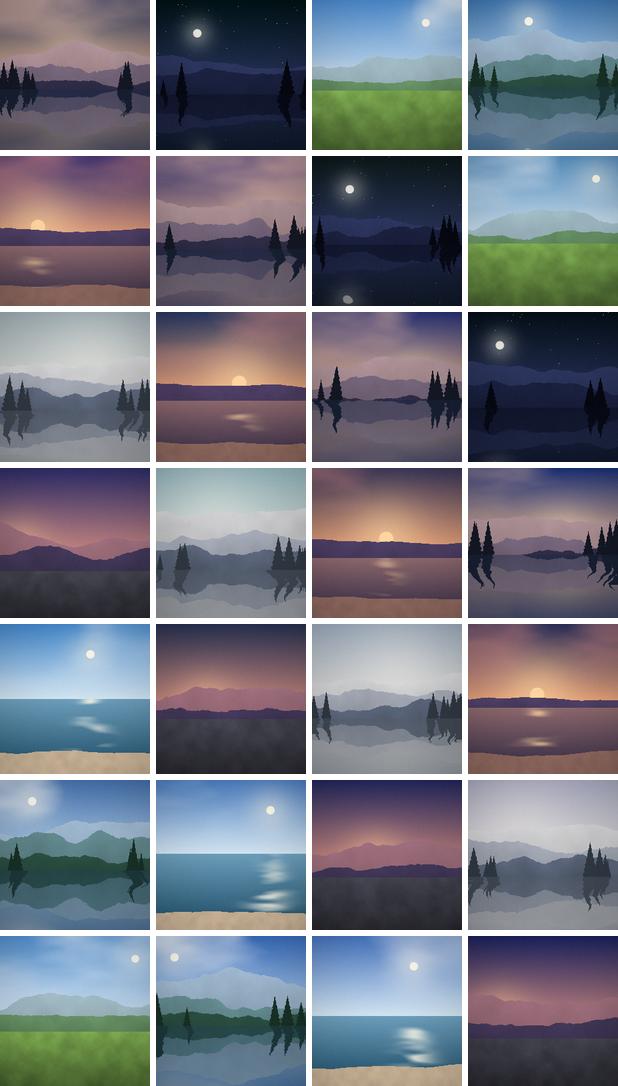
\includegraphics[width=2.94cm]{gallery.png}};
    \fill[white] (1.58,6.36) rectangle (4.52,7.1);
    \fill[white,opacity=0.92] (1.58,1.2) rectangle (4.52,1.55);
  \end{scope}
  \fill[ink,rounded corners=2pt] (2.8,6.93) rectangle (3.3,7.02);
  \node[anchor=west,font=\tiny\bfseries,text=ink] at (1.68,6.97) {9:41};
  \draw[ink,line width=0.4pt] (4.05,6.92) rectangle (4.33,7.02);
  \fill[teal] (4.07,6.94) rectangle (4.1,7.0);
  \node[anchor=west,font=\scriptsize\bfseries,text=ink] at (1.66,6.6) {Photos};
  \node[anchor=east,font=\tiny,text=slate] at (4.46,6.6) {20,000 items};
  \fill[slate!60,rounded corners=1pt] (2.6,1.3) rectangle (3.5,1.36);
}
% dims the screen (for the alert state)
\newcommand{\phonedim}{%
  \begin{scope}
    \clip[rounded corners=7pt] (1.58,1.2) rectangle (4.52,7.1);
    \fill[ink,opacity=0.45] (1.58,1.2) rectangle (4.52,7.1);
  \end{scope}}
% the storage-full popup
\newcommand{\storagealert}{%
  \fill[white,rounded corners=5pt] (1.78,3.15) rectangle (4.32,5.35);
  \draw[teal,line width=0.8pt,rounded corners=5pt] (1.78,3.15) rectangle (4.32,5.35);
  \fill[teal] (3.05,5.0) -- ++(-0.2,-0.35) -- ++(0.4,0) -- cycle;
  \node[font=\tiny\bfseries,text=white] at (3.05,4.77) {!};
  \node[font=\scriptsize\bfseries,text=ink] at (3.05,4.38) {Storage Almost Full};
  \node[font=\tiny,text=slate,align=center] at (3.05,4.0) {127.6 GB of 128 GB used};
  \fill[slate!15,rounded corners=1pt] (2.05,3.62) rectangle (4.05,3.72);
  \fill[teal,rounded corners=1pt] (2.05,3.62) rectangle (4.0,3.72);
  \node[font=\tiny\bfseries,text=steel] at (3.05,3.35) {Manage Storage};}

\newcommand{\cmark}{\ding{51}}
\newcommand{\xmark}{\ding{55}}

\title{Variational Autoencoder}
% slides: no hyphenation, ragged text
\hyphenpenalty=10000 \exhyphenpenalty=10000

\begin{document}

% =================================================================
%  TITLE SLIDE  (deck opener — Part 1 starts the presentation)
% =================================================================

\begin{frame}[plain]

\begin{tikzpicture}[remember picture,overlay,shift={(current page.south west)}]
  \clip (0,0) rectangle (16,9);

  % ---------- slight background tint ----------
  \fill[steel!7] (0,0) rectangle (16,9);

  % ---------- text (centred) ----------
  \node[font=\small\bfseries,text=teal] at (8,7.1) {CSE200 \;\textbullet\; B2 \;\textbullet\; Group 2};
  \node[text=navy,align=center,font=\fontsize{32}{35}\fontseries{eb}\selectfont]
       at (8,5.5) {VARIATIONAL\\AUTOENCODER};
  \node[text=slate,font=\small] at (8,3.3) {Presented by};
  \node[text=ink,font=\small\bfseries] at (8,2.8)
       {Mahir Mahtab \;\textbullet\; Nusaiba Nehleen Bhuiyan \;\textbullet\; Ramisa Musarrat Sujana};
  \node[text=slate,font=\footnotesize\itshape] at (8,2.05) {Department of CSE, BUET};
\end{tikzpicture}
\end{frame}

% =================================================================
%  PAGE 1 — The problem: storage full
% =================================================================
% ---- Slide 1: phone + count ----
\begin{frame}{The Problem: Storage Almost Full}
\begin{canvas}
  \begin{scope}[shift={(2.45,0)}] \phonemockup \end{scope}
\node[anchor=base west,text=navy,font=\fontsize{44}{44}\fontseries{eb}\selectfont] (num) at (7.5,3.5) {20{,}000};
  \node[anchor=base west,text=steel,font=\Large] at ($(num.base east)+(0.11,0.3)$) {photos};
    \node[anchor=north west,text width=8.6cm,align=left,font=\normalsize,text=ink] at (7.5,5.6)
       {Imagine your phone has};
\end{canvas}
\end{frame}


% ---- Slide 3: storage full alert + highlighted bar ----
\begin{frame}{The Problem: Storage Almost Full}
\begin{canvas}
  \begin{scope}[shift={(2.45,0)}]
    \phonemockup
    \phonedim
    \storagealert
  \end{scope}

\node[anchor=base west,text=steel,font=\fontsize{20}{20}\selectfont] (num) at (7.5,4.9) {Storage Almost \textbf{\textcolor{navy}{Full!}}};

  \begin{scope}[shift={(1.6,0)}]
    % storage bar
    \node[anchor=west,font=\footnotesize\bfseries,text=ink] at (5.9,4.12) {Storage};
    \only<1>{\node[anchor=east,font=\footnotesize,text=slate] at (12.9,4.12)
      {127.6 GB of 128 GB used};}
    \only<2->{\node[anchor=east,font=\footnotesize,text=slate] at (12.9,4.12)
      {127.6 GB used \hspace{0.35cm} \textcolor{teal}{\textbf{only 0.4 GB free}}};}

    \begin{scope}[focus on=<2>]
      \fill[navy]     (5.9,3.5) rectangle (11.4,3.8);
      \fill[steel]    (11.4,3.5) rectangle (12.15,3.8);
      \fill[slate!70] (12.15,3.5) rectangle (12.6,3.8);
      \draw[slate!60,line width=0.6pt,rounded corners=2pt] (5.9,3.5) rectangle (12.9,3.8);
    \end{scope}
    \draw[teal,line width=1.3pt,rounded corners=2pt,visible on=<2>] (5.9,3.5) rectangle (12.9,3.8);
\foreach \c/\t/\x in {navy/Photos \, 112 GB/5.9, steel/Apps \, 10 GB/8.5, slate!70/System \, 5.6 GB/10.7}{
  \fill[\c] (\x,3.1) rectangle ++(0.2,0.2);
  \node[anchor=west,font=\scriptsize,text=slate] at (\x+0.26,3.2) {\t};}
  \end{scope}

\node[visible on=<2->,draw=teal,line width=1.2pt,rounded corners=4pt,
      top color=teal!15,bottom color=teal!2,
      inner sep=8pt,text=ink,align=center] at (10.75,2.0)
     {\Large\textbf{\textcolor{teal}{90\% Storage}}\\[4pt]\normalsize Occupied by Photos!};

\end{canvas}
\end{frame}

% ---- Slide 4: what do you do? ----
\begin{frame}{The Problem: Storage Almost Full}
\begin{canvas}
  % ---------- title with accent underline ----------
  \node[font=\fontsize{30}{30}\fontseries{eb}\selectfont,text=navy] (title) at (8,6.3) {What do you do?};

  % ---------- option 1: delete memories ----------
  \begin{scope}[visible on=<2->]
    % soft shadow
    \fill[ink!6,rounded corners=6pt] (3.05,3.85) rectangle (13.25,5.25);
    \draw[slate!45,line width=0.8pt,rounded corners=6pt,top color=slate!10,bottom color=white]
         (2.9,4.0) rectangle (13.1,5.4);
    \node[circle,fill=slate!80!black,minimum size=0.8cm,inner sep=0pt] (badge1) at (4.0,4.7) {};
    \node[font=\large\bfseries,text=white] at (badge1) {\xmark};
    \node[anchor=west,align=left,font=\normalsize,text=slate!85!black,text width=8.4cm] at (4.7,4.7)
         {\textbf{Delete Photos}\\[1pt]{\footnotesize not ideal: once gone, they're gone forever}};
  \end{scope}

  % ---------- option 2: smarter solution ----------
  \begin{scope}[visible on=<3->]
    \fill[ink!10,rounded corners=6pt] (3.05,2.05) rectangle (13.25,3.45);
    \draw[teal,line width=1.2pt,rounded corners=6pt,top color=teal!18,bottom color=white]
         (2.9,2.2) rectangle (13.1,3.6);
    \node[circle,fill=teal,minimum size=0.8cm,inner sep=0pt] (badge2) at (4.0,2.9) {};
    \node[font=\large\bfseries,text=white] at (badge2) {\cmark};
    \node[anchor=west,align=left,font=\normalsize,text=ink,text width=8.4cm] at (4.7,2.9)
         {\textbf{\textcolor{teal}{A Smarter Solution}}\\[1pt]{\footnotesize keep every photo, but use lesser space}};
  \end{scope}
\end{canvas}
\end{frame}


% =================================================================
%  PAGE 2 — Smarter solution: compress
% =================================================================
\begin{frame}{Compression Saves Storage}
\begin{canvas}
  % ---------- flow chart ----------
  \begin{scope}
    \node[draw=slate!60,line width=0.7pt,rounded corners=3pt,fill=white,minimum width=2.9cm,minimum height=0.8cm,
          font=\footnotesize,text=ink] (fa) at (4.1,6.6) {\hspace{0.45cm}   Photo \textbf{(2.8 MB)}};
    \node[draw=slate!60,line width=0.7pt,rounded corners=3pt,fill=white,minimum width=2.9cm,minimum height=0.8cm,
          font=\footnotesize,text=ink] (fb) at (11.9,6.6) {\hspace{0.45cm}   Photo \textbf{(180 KB)}};
    \foreach \p in {fa,fb}{
      \begin{scope}[shift={($(\p.west)+(0.25,-0.17)$)}]
        \draw[slate,line width=0.5pt] (0,0) rectangle (0.42,0.34);
        \fill[slate!70] (0.03,0.03) -- (0.15,0.2) -- (0.24,0.1) -- (0.3,0.16) -- (0.39,0.03) -- cycle;
        \fill[slate!70] (0.3,0.25) circle (0.035);
      \end{scope}}
    \node[mystery,minimum width=1.5cm,minimum height=0.9cm,font=\Large\fontseries{eb}\selectfont,emphasis on=<2->]
         (fm) at (8,6.6) {?};
    \draw[arr] (fa) -- (fm);
    \draw[arr] (fm) -- (fb);
  \end{scope}

  % ---------- real photos ----------
  \only<2->{\begin{scope}
    \node[inner sep=0pt] (po) at (3.9,3.95) {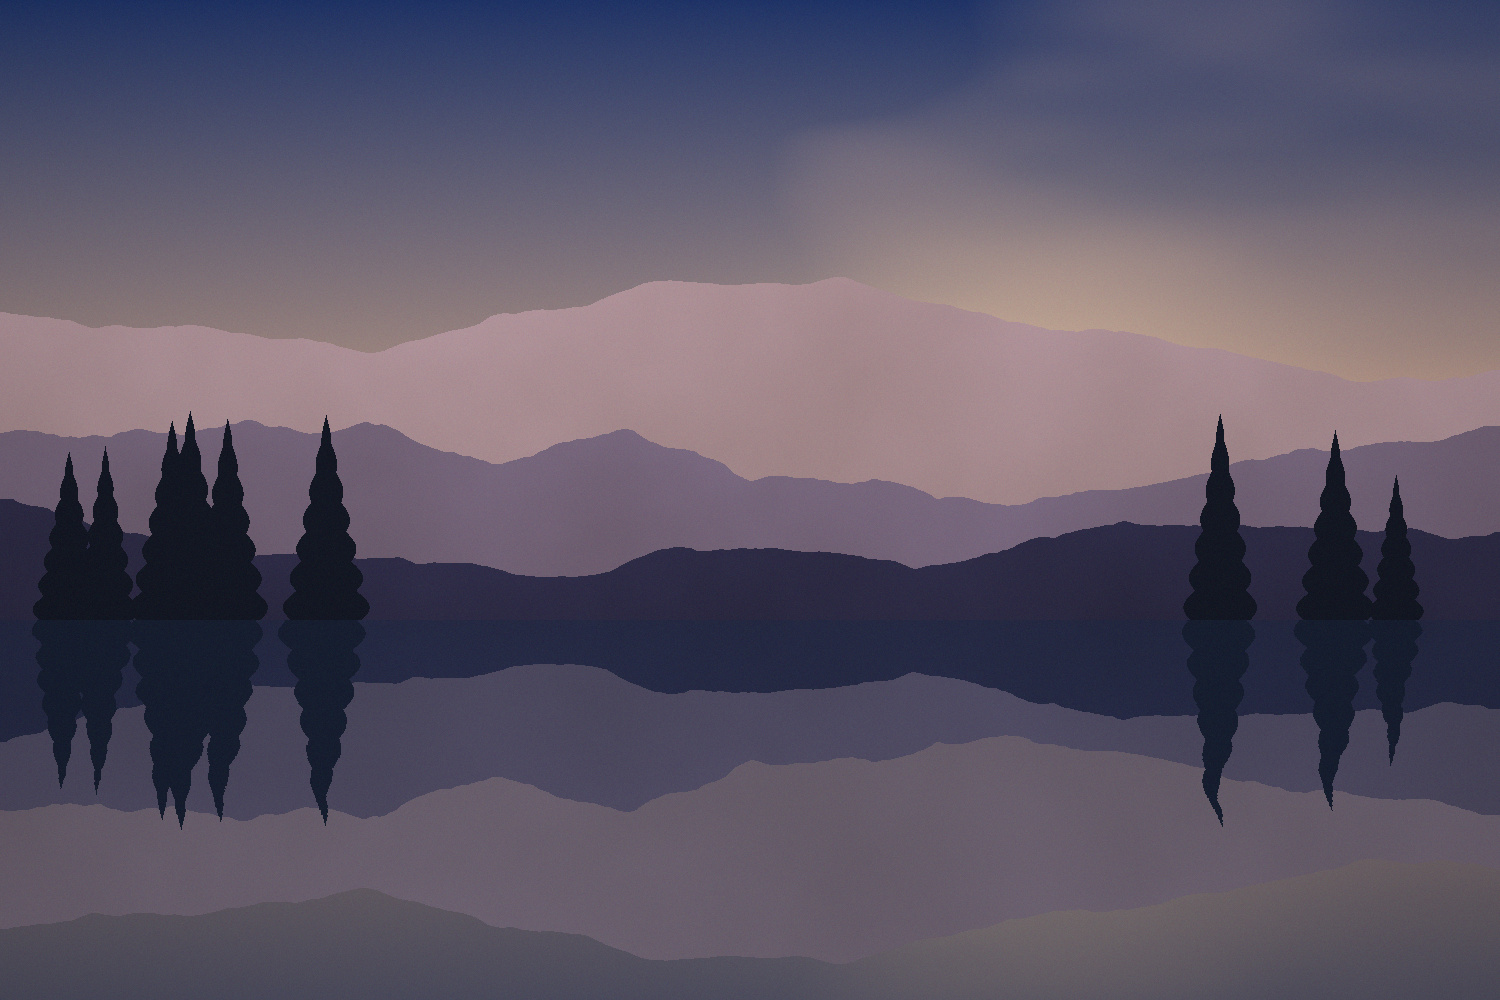
\includegraphics[width=4.5cm]{photo_original.jpg}};
    \draw[photo] (po.south west) rectangle (po.north east);
    \node[inner sep=0pt] (pc) at (12.1,3.95) {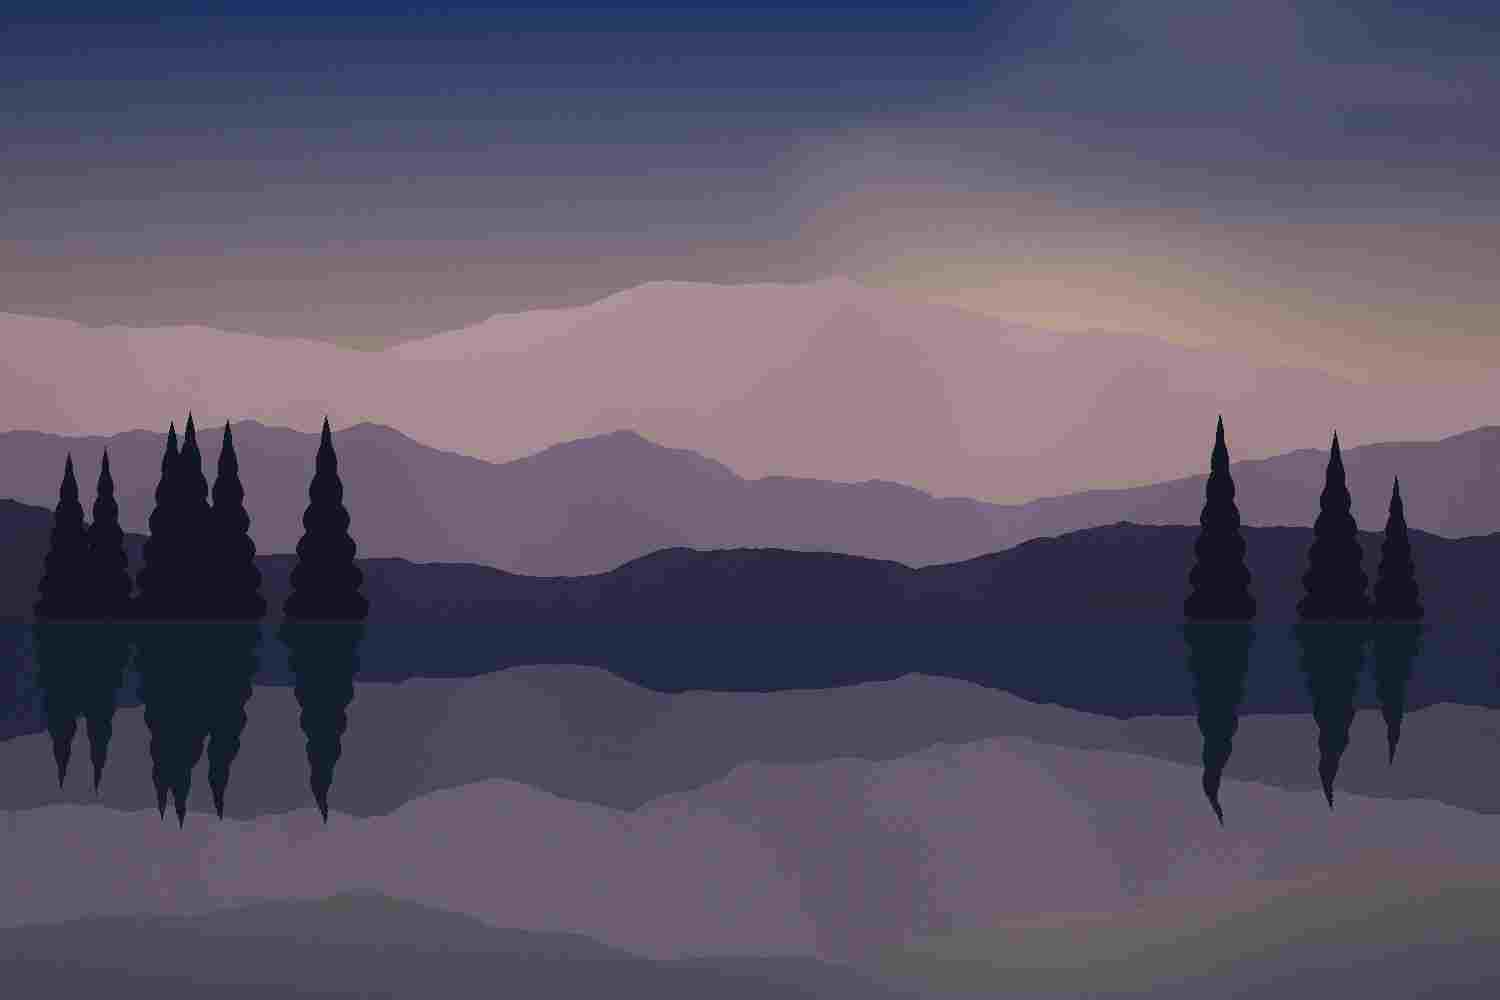
\includegraphics[width=4.5cm]{photo_compressed.jpg}};
    \draw[photo] (pc.south west) rectangle (pc.north east);
    \node[mystery,minimum width=1.9cm,minimum height=1.5cm,emphasis on=<2->] (pm) at (8,3.95) {?};
    \draw[arr] (po) -- (pm);
    \draw[arr] (pm) -- (pc);
    \node[lbl,anchor=north] at (po.south) {original \;\textbullet\; \textbf{2.8 MB}};
    \node[lbl,anchor=north] at (pc.south) {compressed \;\textbullet\; \textbf{180 KB} \;\textcolor{teal}{($\approx$15$\times$ smaller)}};

    \node[font=\normalsize,text=ink,align=center] at (8,1.3)
       {Compressed image is \textbf{\textcolor{deepteal}{15 times smaller}}};

  \end{scope}}


\end{canvas}
\end{frame}

% =================================================================
%  PAGE 3 — Enter the autoencoder
% =================================================================
\begin{frame}{Enter the Autoencoder}
\begin{canvas}
  \only<1-2>{%
    \node[inner sep=0pt] (po) at (3.3,4.5) {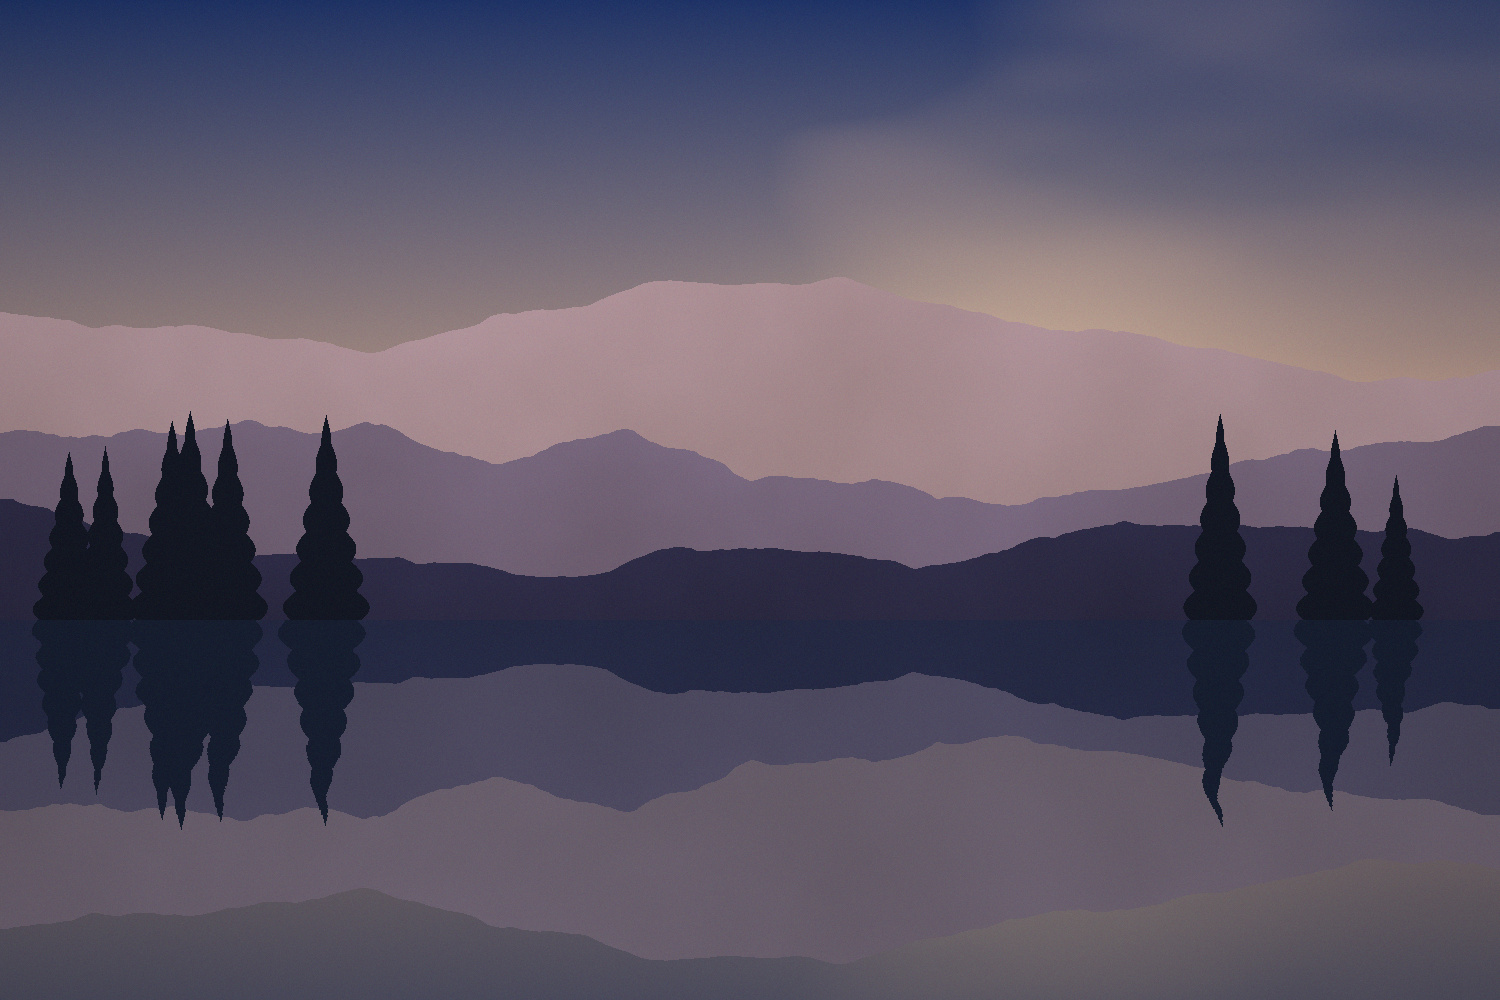
\includegraphics[width=3.9cm]{photo_original.jpg}};
    \draw[photo] (po.south west) rectangle (po.north east);
    \node[inner sep=0pt] (pc) at (12.7,4.5) {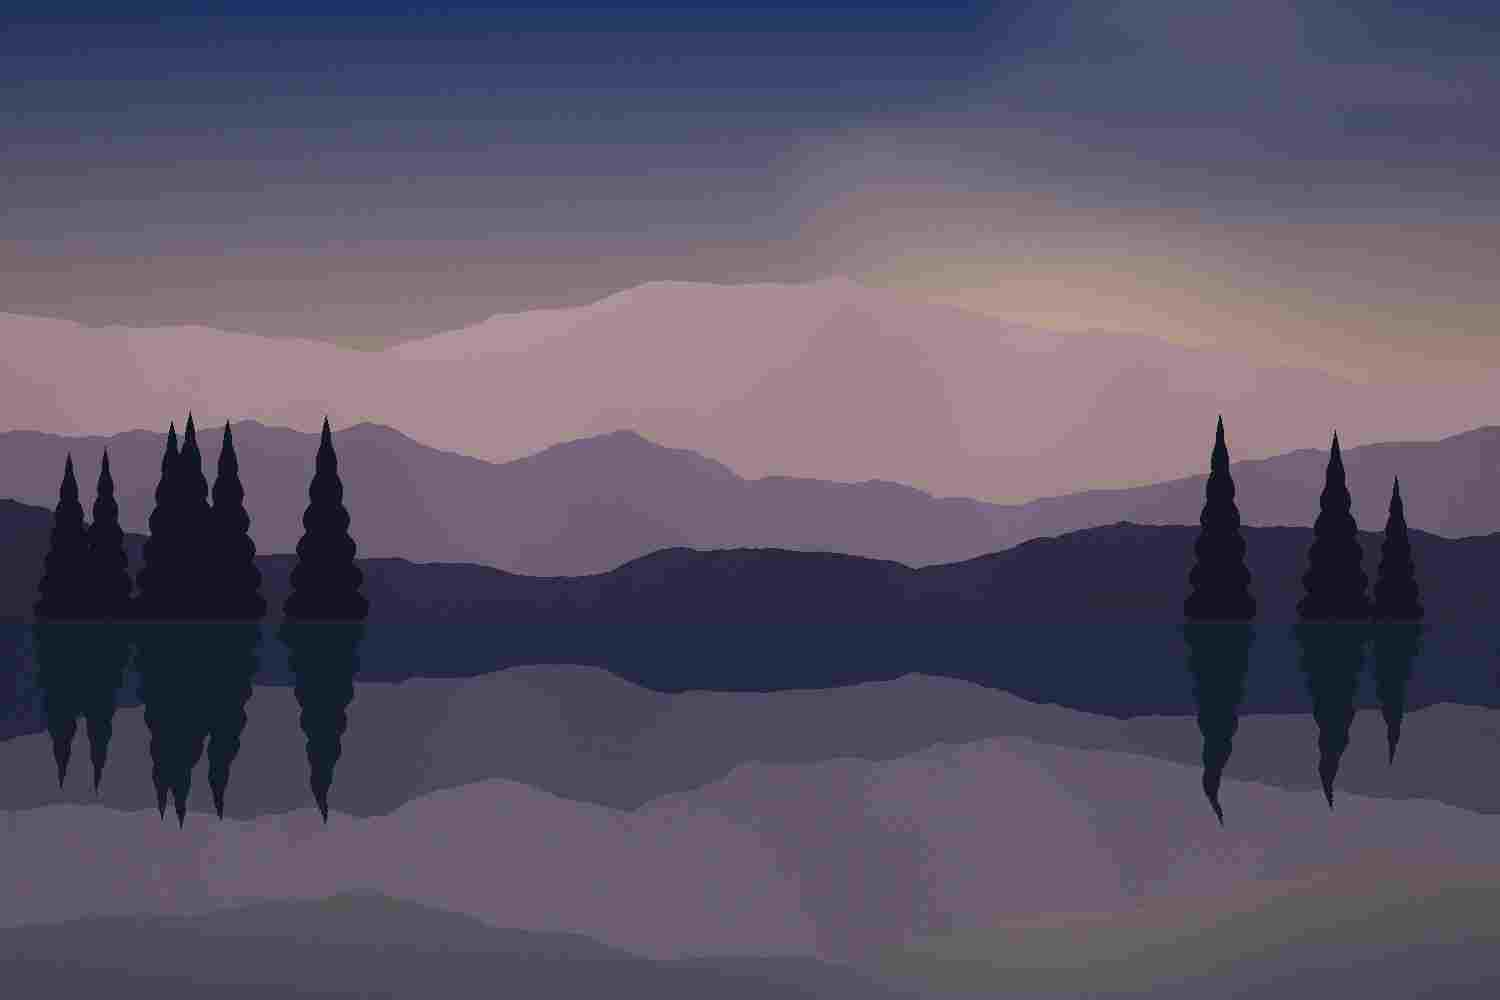
\includegraphics[width=3.9cm]{photo_compressed.jpg}};
    \draw[photo] (pc.south west) rectangle (pc.north east);
    \node[lbl,anchor=north] at (po.south) {2.8 MB};
    \node[lbl,anchor=north] at (pc.south) {180 KB};
    \draw[arr] (po) -- (8-1.95,4.5);
    \draw[arr] (8+1.95,4.5) -- (pc);

    \node[mystery,minimum width=3.9cm,minimum height=2.6cm,emphasis on=<1>,
          alt=<2>{draw=navy,line width=1pt}{}] (box) at (8,4.5) {};
    \node[visible on=<1>,text=deepteal,font=\fontsize{40}{40}\fontseries{eb}\selectfont] at (box) {?};

    \only<1>{\node[font=\large,text=ink,align=center] at (8,2.0)
       {What goes inside the \textbf{\textcolor{deepteal}{mysterious middle box}}?};}

    \begin{scope}[visible on=<2>]
      \node[text=navy,font=\large\fontseries{eb}\selectfont] at (8,5.3) {Autoencoder};
      \fill[steel!12] (6.55,4.85) -- (7.65,4.45) -- (7.65,3.95) -- (6.55,3.55) -- cycle;
      \draw[steel,line width=0.8pt] (6.55,4.85) -- (7.65,4.45) -- (7.65,3.95) -- (6.55,3.55) -- cycle;
      \fill[teal!10] (9.45,4.85) -- (8.35,4.45) -- (8.35,3.95) -- (9.45,3.55) -- cycle;
      \draw[teal,line width=0.8pt] (9.45,4.85) -- (8.35,4.45) -- (8.35,3.95) -- (9.45,3.55) -- cycle;
      \node[rectangle,fill=navy!8,draw=navy,line width=0.8pt,minimum width=0.42cm,minimum height=0.5cm,
            inner sep=0pt,font=\scriptsize,text=navy] at (8,4.2) {$z$};
      \draw[slate,line width=0.6pt,->,>={Stealth[length=1.3mm]}] (7.65,4.2) -- (7.79,4.2);
      \draw[slate,line width=0.6pt,->,>={Stealth[length=1.3mm]}] (8.21,4.2) -- (8.35,4.2);
      \node[font=\tiny,text=steel] at (7.0,3.35) {encoder};
      \node[font=\tiny,text=teal!80!black] at (9.0,3.35) {decoder};
    \end{scope}

    \node[visible on=<2>,font=\large,text=ink,align=center] at (8,2.0)
         {This box is exactly where \textbf{\textcolor{navy}{autoencoders}} come in.};
  }
  % ---------- step 3: big standalone autoencoder diagram ----------
  \begin{scope}[visible on=<3->]
    \node[draw=navy,line width=1.3pt,rounded corners=5pt,fill=white,
          minimum width=6.2cm,minimum height=4.13cm] (bigbox) at (8,4.7) {};
    \node[text=navy,font=\Large\fontseries{eb}\selectfont] at (8,5.97) {Autoencoder};

    \fill[steel!12] (5.69,5.26) -- (7.44,4.62) -- (7.44,3.83) -- (5.69,3.19) -- cycle;
    \draw[steel,line width=1.2pt] (5.69,5.26) -- (7.44,4.62) -- (7.44,3.83) -- (5.69,3.19) -- cycle;
    \fill[teal!10] (10.31,5.26) -- (8.56,4.62) -- (8.56,3.83) -- (10.31,3.19) -- cycle;
    \draw[teal,line width=1.2pt] (10.31,5.26) -- (8.56,4.62) -- (8.56,3.83) -- (10.31,3.19) -- cycle;
    \node[rectangle,fill=navy!8,draw=navy,line width=1.2pt,minimum width=0.67cm,minimum height=0.8cm,
          inner sep=0pt,font=\normalsize,text=navy] at (8,4.22) {$z$};
    \draw[slate,line width=1pt,->,>={Stealth[length=2mm]}] (7.44,4.22) -- (7.67,4.22);
    \draw[slate,line width=1pt,->,>={Stealth[length=2mm]}] (8.33,4.22) -- (8.56,4.22);
    \node[font=\normalsize,text=steel] at (6.41,2.87) {encoder};
    \node[font=\normalsize,text=teal!80!black] at (9.59,2.87) {decoder};
  \end{scope}

  \node[visible on=<3->,font=\large,text=ink,align=center] at (8,2.0)
       {A neural network that learns to \textcolor{steel}{\textbf{compress}} data and \textcolor{teal}{\textbf{reconstruct}} it};

  \node[visible on=<3->,lbl, font = \normalsize] at (8,1.45)
       {It has two main parts: \textcolor{steel}{\textbf{1. Encoder }} \textcolor{teal}{\textbf{2. Decoder}}};
\end{canvas}
\end{frame}

% =================================================================
%  PAGE 4 — Autoencoder architecture
% =================================================================
\begin{frame}{Autoencoder Architecture}
\begin{canvas}
  % layers: x positions and node counts
  \def\LA{4.3}\def\LB{6.05}\def\LC{7.95}\def\LD{9.85}\def\LE{11.6}
  \def\yc{4.45}

  % bottleneck band
  \draw[fill=navy!5,draw=navy!35,line width=0.6pt,dashed,rounded corners=4pt,visible on=<2->,focus on=<2>]
       (7.35,2.75) rectangle (8.55,6.15);
  \node[visible on=<2->,font=\scriptsize\bfseries,text=navy] at (7.95,5.85) {bottleneck};
  \node[visible on=<2->,font=\scriptsize,text=navy,align=center] at (7.95,3.05) {code $z$};

  % nodes
  \begin{scope}[visible on=<1->]
    \foreach \i in {1,...,5} \node[neuron,fill=steel!12,draw=steel,text=navy] (a\i) at (\LA,{\yc+(3-\i)*0.75}) {$x_{\i}$};
    \foreach \i in {1,...,3} \node[neuron,fill=steel!12,draw=steel] (b\i) at (\LB,{\yc+(2-\i)*0.75}) {};
    \foreach \i in {1,...,2} \node[neuron,fill=navy!8,draw=navy,text=navy] (c\i) at (\LC,{\yc+(1.5-\i)*0.8}) {$z_{\i}$};
    \foreach \i in {1,...,5} \foreach \j in {1,...,3} \draw[slate!45,line width=0.35pt] (a\i) -- (b\j);
    \foreach \i in {1,...,3} \foreach \j in {1,...,2} \draw[slate!45,line width=0.35pt] (b\i) -- (c\j);
    \node[inner sep=0pt] (xin) at (2.0,\yc) {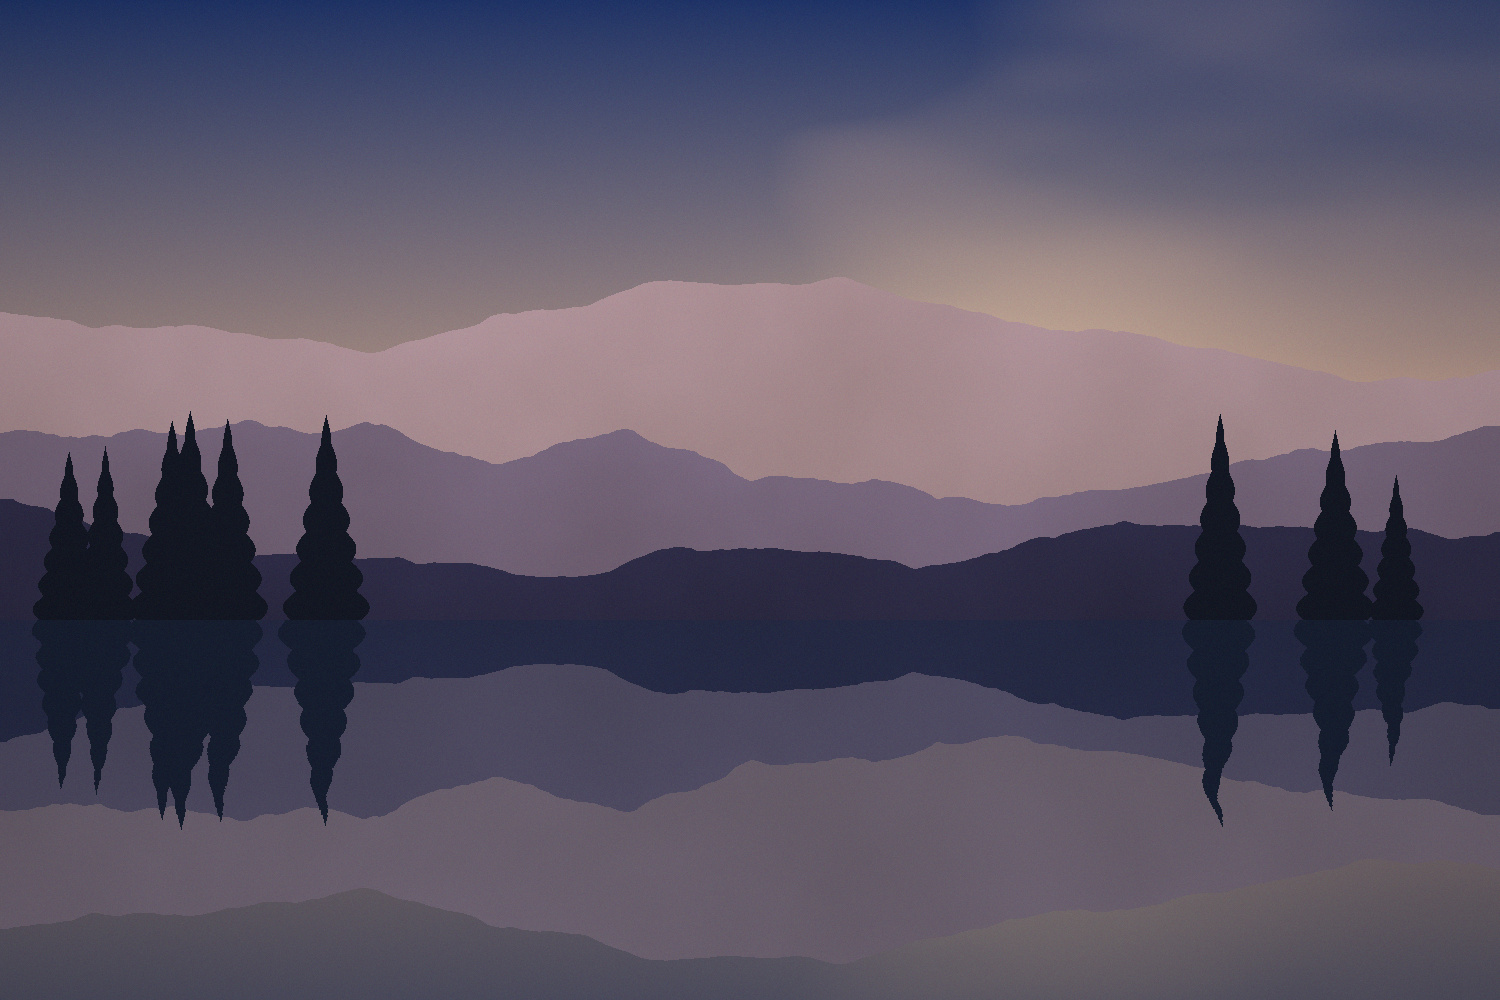
\includegraphics[width=2.1cm]{photo_original.jpg}};
    \draw[photo] (xin.south west) rectangle (xin.north east);
    \node[lbl,anchor=north] at (xin.south) {input $x$};
    \draw[arr] (xin.east) -- ++(0.9,0);
    \draw[decorate,decoration={brace,amplitude=6pt},steel,line width=0.8pt] (4.0,6.4) -- (7.4,6.4)
         node[midway,above=6pt,font=\footnotesize\bfseries,text=steel] {\ding{172}\; Encoder};
  \end{scope}
  \begin{scope}[visible on=<3->]
    \foreach \i in {1,...,3} \node[neuron,fill=teal!10,draw=teal] (d\i) at (\LD,{\yc+(2-\i)*0.75}) {};
    \foreach \i in {1,...,5} \node[neuron,fill=teal!10,draw=teal,text=teal!70!black] (e\i) at (\LE,{\yc+(3-\i)*0.75}) {$\hat{x}_{\i}$};
    \foreach \i in {1,...,2} \foreach \j in {1,...,3} \draw[slate!45,line width=0.35pt] (c\i) -- (d\j);
    \foreach \i in {1,...,3} \foreach \j in {1,...,5} \draw[slate!45,line width=0.35pt] (d\i) -- (e\j);
    \node[inner sep=0pt] (xout) at (13.9,\yc) {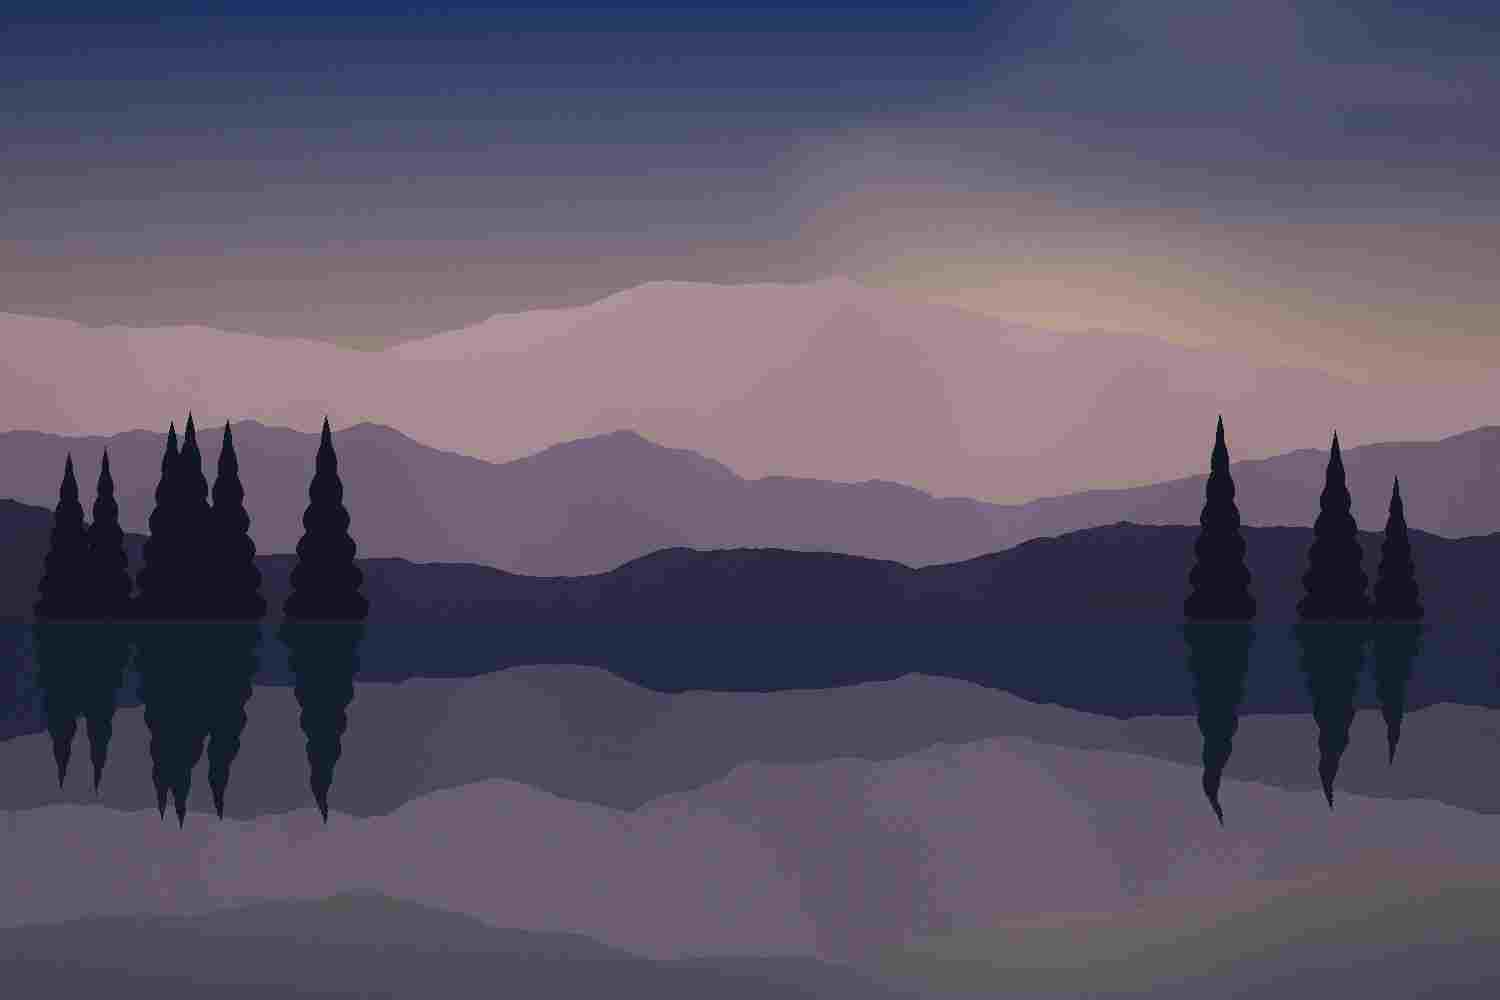
\includegraphics[width=2.1cm]{photo_compressed.jpg}};
    \draw[photo] (xout.south west) rectangle (xout.north east);
    \node[lbl,anchor=north] at (xout.south) {reconstruction $\hat{x}$};
    \draw[arr] (11.9,\yc) -- (xout.west);
    \draw[decorate,decoration={brace,amplitude=6pt},teal,line width=0.8pt] (8.5,6.4) -- (11.9,6.4)
         node[midway,above=6pt,font=\footnotesize\bfseries,text=teal!80!black] {\ding{173}\; Decoder};
  \end{scope}
  % redraw node layer on top of edges
  \begin{scope}[visible on=<1->]
    \foreach \i in {1,...,2} \node[neuron,fill=navy!8,draw=navy,text=navy] at (c\i) {$z_{\i}$};
  \end{scope}

  % explanation
  \node[font=\normalsize,text=ink,align=center,text width=13cm] at (8,1.55) {%
    \only<1>{The \textbf{\textcolor{steel}{encoder}} compresses the image, layer by layer, until it reaches the bottleneck.}%
    \only<2>{The \textbf{\textcolor{navy}{bottleneck}} allows only the \emph{essential} information to pass which is called \emph{\textcolor{navy}{latent code}}, represented in the \emph{\textcolor{navy}{latent space}} }%
    \only<3>{The \textbf{\textcolor{teal}{decoder}} uses that latent code to rebuild the image: \; $\hat{x}\approx x$.}};
\end{canvas}
\end{frame}
% =================================================================
%  PAGE 5 — Latent space: islands and gaps
% =================================================================
\begin{frame}{The Problem with Autoencoders}
\begin{canvas}
  \begin{scope}[shift={(4.65,4.1)}]
    \latentpanel
    \clusters{0}{1}
  \only<1,3>{\clusterlabels{1}}
  \only<2>{%
    \foreach \cx/\cy/\dx/\dy/\d in {-2.35/1.55/-0.95/0.25/0, -0.25/1.85/0.55/0.3/1, 2.20/1.20/0.2/0.8/7,
                                    -2.05/-1.35/0.9/-0.5/3, 0.60/-0.45/-0.8/-0.5/5, 2.40/-1.65/-0.15/-0.75/9}
      {\thumb[minimum size=0.62cm,draw=teal,line width=1pt,fill=teal!10,
              font=\normalsize\fontseries{eb}\selectfont,text=teal!80!black]{\cx+\dx,\cy+\dy}{\d}}
  }
    % step 2: one dot = one image
    \begin{scope}[visible on=<1>]
      \draw[sky,line width=0.9pt] (2.2,1.2) circle (0.14);
      \draw[sky,line width=0.6pt] (2.33,1.15) -- (2.85,0.05);
      \node[fill=white,draw=sky,line width=0.9pt,rounded corners=3pt,font=\normalsize,text=sky!70!black,
            inner sep=5pt,anchor=west] at (2.95,-0.05) {\textbf{1 dot = 1 image}};
    \end{scope}
    % step 3: highlight gaps
    \begin{scope}[visible on=<3->]
      \foreach \x/\y/\r in {-1.25/0.3/0.55, 1.3/0.2/0.5, -0.5/-1.95/0.45, 1.0/2.2/0.32, 3.1/-0.1/0.4}
        \draw[slate,line width=0.6pt,dash pattern=on 2pt off 1.6pt] (\x,\y) circle (\r);
      \node[font=\scriptsize\itshape,text=slate] at (-1.25,0.3) {empty};
      \node[font=\scriptsize\itshape,text=slate] at (1.3,0.2) {empty};
    \end{scope}
  \end{scope}

  % right-hand explanation
  \node[anchor=north west,text width=6.2cm,align=left,font=\normalsize,text=ink] at (8.95,6.9) {%
    Here in this bottleneck space, each point is exactly \textbf{one image} after compression};
  \node[anchor=north west,text width=6.2cm,align=left,font=\normalsize,text=ink,visible on=<2->] at (8.95,5.2) {%
    Notice how similar images form separate \textbf{\textcolor{navy}{islands}}, such as 0, 1, 5, 7, and 9};
  \node[anchor=north west,text width=6.2cm,align=left,font=\normalsize,text=ink,visible on=<3->] at (8.95,3.5) {%
     There are lots of \textbf{\textcolor{teal}{empty spaces}} between them. The decoder has not seen training examples from these regions.};
\end{canvas}
\end{frame}

% =================================================================
%  PAGE 6 — Sampling from a gap
% =================================================================
\begin{frame}{What Lives in the Gaps?}
\begin{canvas}
  \begin{scope}[shift={(4.65,4.1)}]
    \latentpanel
    \clusters{0}{1}
        \foreach \cx/\cy/\dx/\dy/\d in {-2.35/1.55/-0.95/0.25/0, -0.25/1.85/0.55/0.3/1, 2.20/1.20/0.2/0.8/7,
                                    -2.05/-1.35/0.9/-0.5/3, 0.60/-0.45/-0.8/-0.5/5, 2.40/-1.65/-0.15/-0.75/9}
      {\thumb[minimum size=0.62cm,draw=teal,line width=1pt,fill=teal!10,
              font=\normalsize\fontseries{eb}\selectfont,text=teal!80!black]{\cx+\dx,\cy+\dy}{\d}}
    % A: inside an island    
    \draw[navy,line width=1pt] (2.2,1.2) circle (0.16);
    \draw[navy,line width=0.6pt] (2.34,1.14) -- (3.15,0.7);
    \node[fill=white,draw=navy,line width=0.9pt,rounded corners=3pt,font=\normalsize,text=navy,
          inner sep=4pt,anchor=west] at (3.25,0.7) {\textbf{A}};
    % B: in an empty region
    \begin{scope}[visible on=<2->]
      \draw[teal,line width=0.6pt,dash pattern=on 2pt off 1.6pt] (-1.25,0.3) circle (0.5);
      \node[star,star points=5,star point ratio=2.3,fill=navy,inner sep=1.4pt] at (-1.25,0.3) {};
      \draw[navy,line width=0.6pt] (-0.75,0.3) -- (-0.35,0.3);
      \node[fill=white,draw=navy,line width=0.9pt,rounded corners=3pt,font=\normalsize,text=navy!80!black,
            inner sep=4pt,anchor=west] at (-0.25,0.3) {\textbf{B}};
    \end{scope}
  \end{scope}

  % right: decode A and B
  \tikzset{smalldec/.style={dec,minimum width=1.1cm,minimum height=1.0cm,inner sep=1pt,font=\tiny\bfseries}}
  \node[font=\footnotesize,text=navy,anchor=west] at (8.95,6.95) {\textbf{A}\; point inside an island};
  \node[smalldec] (dA) at (11.2,5.95) {Decoder};
  \draw[arr] (9.3,5.95) -- (dA.west);
  \thumb[minimum size=1.1cm,font=\huge\fontseries{eb}\selectfont]{13.25,5.95}{7}
  \draw[arr] (dA.east) -- (12.65,5.95);
  \node[font=\footnotesize,text=navy,anchor=north] at (13.25,5.33) {\cmark\ a clear ``7''};


  \begin{scope}[visible on=<2->]
    \node[font=\footnotesize,text=teal!80!black,anchor=west] at (8.95,3.6) {\textbf{B}\; random point from an empty gap};
    \node[smalldec] (dB) at (11.2,2.6) {Decoder};
    \draw[arr] (9.3,2.6) -- (dB.west);
      \thumb[minimum size=1.1cm,font=\huge\fontseries{eb}\selectfont]{13.25,2.75}{?}
    \garbled{13.25,2.6}{1.1}
    \draw[arr] (dB.east) -- (12.65,2.6);
    \node[font=\footnotesize,text=teal!80!black,anchor=north] at (13.25,1.98) {\xmark\ meaningless};
  \end{scope}

\end{canvas}
\end{frame}

% =================================================================
%  PAGE — A new idea
% =================================================================
\begin{frame}{The Key Insight}
\begin{canvas}
  % ---------- the question ----------
  \fill[ink!8,rounded corners=6pt] (2.95,4.0) rectangle (13.15,6.05);
  \draw[steel,line width=1.2pt,rounded corners=6pt,top color=steel!12,bottom color=white]
       (2.8,4.15) rectangle (13.0,6.2);
  \node[text width=8.8cm,align=center,font=\large,text=ink] at (7.9,5.18) {%
    Instead of storing each image as one exact point, what if every image were represented as a \textbf{\textcolor{steel}{distribution}}?};

  % ---------- the answer ----------
      \begin{scope}[visible on=<2->]
    \fill[ink!10,rounded corners=6pt] (2.95,1.85) rectangle (13.15,3.6);
    \draw[teal,line width=1.4pt,rounded corners=6pt,top color=teal!18,bottom color=white]
         (2.8,2.0) rectangle (13.0,3.75);
    \node[text width=9.2cm,align=center,font=\large\bfseries,text=teal] at (7.9,2.88) {%
      That's the core idea behind the \textcolor{teal!60!navy}{Variational Autoencoder (VAE)}};
  \end{scope}
\end{canvas}
\end{frame}
% =================================================================
%  PAGE 7 — From points to distributions
% =================================================================
\begin{frame}{From Points to Distributions}
\begin{canvas}
  \begin{scope}[shift={(4.65,4.1)}]
    \latentpanel
    \begin{scope}
      \clip (-3.7,-2.95) rectangle (3.7,2.95);
      \only<1>{\clusters{0}{1}}
      \only<2>{\clusters{0.24}{1}}
      \only<3->{\clusters{0.42}{0.7}}
    \end{scope}
    \only<1-2>{\clusterlabels{1}}
    \only<3->{%
      \node[star,star points=5,star point ratio=2.3,fill=teal,inner sep=1.4pt] (new) at (-0.55,0.35) {};
      \draw[teal,line width=0.6pt] (new) -- (-2.2,-2.45)
        node[fill=white,draw=teal,rounded corners=2pt,inner sep=2.5pt,font=\scriptsize,text=teal!80!black,anchor=north west]
        at (-3.55,-2.1) {sampled point $\rightarrow$ plausible image};}
  \end{scope}

  % ---------- morph: one image -> one point / one cloud (slides 1,2 only) ----------
  \only<1,2>{%
    \thumb[minimum size=0.9cm,font=\LARGE\fontseries{eb}\selectfont]{9.6,5.05}{3}
    \node[lbl] at (9.6,4.35) {one image};
    \draw[arr] (10.15,5.05) -- (11.35,5.05);
    \node[lbl,font=\scriptsize] at (10.75,5.3) {encode};
  }
  \coordinate (P) at (12.95,5.05);
  \only<1>{%
    \fill[navy] (P) circle (0.09);
    \node[lbl,text=navy] at ($(P)+(0,-0.7)$) {one exact point};}
  \only<2>{%
    \fill[navy,opacity=0.07] (P) ellipse (1.25 and 0.72);
    \fill[navy,opacity=0.09] (P) ellipse (0.85 and 0.5);
    \fill[navy,opacity=0.12] (P) ellipse (0.48 and 0.28);
    \draw[navy!60,line width=0.5pt,dashed] (P) ellipse (1.25 and 0.72);
    \pgfmathsetseed{9}
    \foreach \k in {1,...,26}{
      \pgfmathsetmacro\rr{min(1.8,sqrt(-2*ln(max(rnd,0.01))))}
      \pgfmathsetmacro\tt{360*rnd}
      \fill[navy!70] ($(P)+({0.45*\rr*cos(\tt)},{0.26*\rr*sin(\tt)})$) circle (0.035);}
    \fill[navy] (P) circle (0.07);
    \draw[steel,line width=0.7pt,<->,>={Stealth[length=1.2mm]}] (P) -- ++(0.85,0)
         node[midway,above=-1pt,font=\scriptsize,text=steel] {$\bm{\sigma}$};
    \node[font=\scriptsize,text=navy] at ($(P)+(-0.2,-0.2)$) {$\bm{\mu}$};
    \node[lbl,text=navy] at ($(P)+(0,-0.98)$) {a small cloud \; $\mathcal{N}(\bm{\mu},\bm{\sigma}^2)$};}

  % ---------- slide 3: text on top ----------
  \only<3>{%
    \node[anchor=north west,text width=5.9cm,align=left,font=\footnotesize,text=ink] at (9.15,6.9) {%
      Notice, the distributions overlap, which \textbf{reduces empty gaps}.\\[10pt]As a result, we can choose a new point from that area and it will still decode into a meaningful image.};
  }

    % ---------- slide 3: flowchart below the text ----------
  \only<3>{%
    \node[draw=teal,line width=0.6pt,rounded corners=3pt,fill=white,minimum width=2.0cm,minimum height=0.75cm,
          font=\footnotesize,text=teal!80!black] (fs1) at (9.6,3.1) {Sample point};
    \node[dec,minimum width=1.6cm,minimum height=0.9cm,inner sep=1pt,font=\small\bfseries] (fs2) at (12.3,3.1) {Decoder};
    \node[draw=slate!50,line width=0.5pt,fill=white,minimum size=1.0cm,inner sep=0pt,text=teal!70!black,
          font=\huge\fontseries{eb}\selectfont] (fs3) at (14.6,3.1) {\checkmark};
    \draw[arr] (fs1) -- (fs2);
    \draw[arr] (fs2) -- (fs3);
    \node[lbl,anchor=north,text=teal!80!black] at (14.6,2.35) {Meaningful\\image};
  }

  % ---------- highlight chips ----------
  \node[chip,draw=teal,anchor=west,text width=5.55cm,inner xsep=5pt,align=left,visible on=<2>,line width=1.1pt] at (9.1,2.9)
       {\textbf{\textcolor{teal}{VAE:}} one image $\rightarrow$ one \textbf{distribution}};

  \only<2>{%
    \node[anchor=north west,text width=5.9cm,align=left,font=\footnotesize,text=ink] at (9.15,2.55) {%
      Each image now occupies a \textbf{small area}.};
  }
\end{canvas}
\end{frame}


% =================================================================
%  PAGE 8 — Smile: value vs distribution  (senior slide 27)
% =================================================================
\begin{frame}{One Image, One Distribution}
\begin{canvas}
  \def\xa{5.0}\def\xb{11.2}\def\W{4.2}
  % headers
  \node[font=\footnotesize\bfseries,text=ink] at (\xa,7.1) {Smile (discrete value)};
  \node[chip,draw=steel,font=\scriptsize] at (\xa,6.62) {$\rightarrow$ \textbf{\textcolor{steel}{Autoencoder}}: a single point};
  \begin{scope}[visible on=<2->]
    \node[font=\footnotesize\bfseries,text=ink] at (\xb,7.1) {Smile (probability distribution)};
    \node[chip,draw=teal,font=\scriptsize,line width=1.1pt] at (\xb,6.62) {$\rightarrow$ \textbf{\textcolor{teal}{Variational Autoencoder}}: a distribution};
    \node[font=\footnotesize\itshape,text=slate] at (8.1,3.8) {vs.};
  \end{scope}
  \node[lbl,rotate=90,font=\scriptsize] at (0.95,3.8) {each row = one image};

  \foreach \y/\s/\skin/\hair/\st/\bg/\shirt/\m/\sg/\h in {
      5.72/-0.5/teal!28!white/teal!75!ink/0/steel!10/sky!45/-0.55/0.26/0.62,
      4.42/0.05/teal!45!white/ink!85/1/slate!12/slate!55/0.0/0.42/0.42,
      3.12/0.6/teal!85!ink/ink/2/teal!12/teal!45/0.5/0.17/0.86,
      1.82/0.9/teal!55!white/slate!55!ink/3/navy!8/steel!60/0.78/0.1/0.95}{
    \face{2.05,\y}{1.02}{\s}{\skin}{\hair}{\st}{\bg}{\shirt}
    \numline{\xa,\y-0.3}{\W}
    \fill[navy] (\xa+\m*\W/2,\y-0.3) circle (0.085);
    \begin{scope}[visible on=<2->]
      \numline{\xb,\y-0.3}{\W}
      \gauss{\xb,\y-0.3}{\W}{\m}{\sg}{\h}
    \end{scope}}
\end{canvas}
\end{frame}

% =================================================================
%  PAGE 9 — Latent attributes as distributions  (senior slide 28)
% =================================================================
\begin{frame}{VAE Simplified: Latent Attributes}
\begin{canvas}
  \def\yc{4.45}
  \person{1.95,\yc}{1.45}
  \node[lbl,anchor=north] at (1.95,3.5) {input $x$};
  \node[enc,minimum width=2.1cm,minimum height=1.3cm,visible on=<1->,focus on=<1>] (en) at (4.25,\yc) {Encoder};
  \node[lbl,visible on=<1->] at (4.25,3.15) {$q_\phi(z\mid x)$};
  \draw[arr] (2.8,\yc) -- (en.west);

  % latent attribute panel
  \begin{scope}[visible on=<2->]
    \draw[slate!45,line width=0.6pt,rounded corners=8pt,fill=white] (5.75,2.1) rectangle (10.25,7.2);
    \draw[arr] (en.east) -- (5.7,\yc);
    \foreach \y/\name/\m/\sg/\h in {6.75/Smile/0.2/0.18/0.42, 5.9/Skin tone/0.05/0.25/0.34, 5.05/Gender/-0.45/0.16/0.46,
                                    4.2/Beard/0.7/0.12/0.52, 3.35/Glasses/-0.35/0.14/0.5, 2.5/Hair colour/0.05/0.12/0.52}{
      \node[anchor=east,font=\scriptsize,text=ink] at (7.3,\y) {\name};
      \numline{8.75,\y-0.05}{2.4}
      \gauss{8.75,\y-0.05}{2.4}{\m}{\sg}{\h}}
    \node[lbl] at (8.0,1.75) {latent attributes: one distribution each};
  \end{scope}

  \begin{scope}[visible on=<3->]
    \node[dec,minimum width=2.1cm,minimum height=1.3cm,focus on=<3>] (de) at (11.75,\yc) {Decoder};
    \node[lbl] at (11.75,3.15) {$p_\theta(x\mid z)$};
    \draw[arr] (10.3,\yc) -- (de.west);
    \person{14.0,\yc}{1.45}
    \node[lbl,anchor=north] at (14.0,3.5) {reconstruction $\hat{x}$};
    \draw[arr] (de.east) -- (13.2,\yc);
  \end{scope}
\end{canvas}
\end{frame}

% =================================================================
%  PAGE 10 — Sample -> reconstruct  (senior slide 29)
% =================================================================
\begin{frame}{VAE Simplified: Sampling and Decoding}
\begin{canvas}
  % compact latent distributions with two samples
  \draw[slate!45,line width=0.6pt,rounded corners=8pt,fill=white] (0.95,1.85) rectangle (4.95,7.15);
  \foreach \y/\name/\m/\sg/\h/\a/\b in {6.7/Smile/0.2/0.18/0.42/0.23/0.17, 5.85/Skin tone/0.05/0.25/0.34/0.02/0.28,
                                        5.0/Gender/-0.15/0.16/0.46/-0.18/-0.11, 4.15/Beard/0.7/0.12/0.52/0.71/0.66,
                                        3.3/Glasses/-0.15/0.14/0.5/-0.19/-0.14, 2.45/Hair colour/0.3/0.12/0.52/0.33/0.26}{
    \node[anchor=west,font=\tiny,text=ink] at (1.05,\y+0.3) {\name};
    \numline{3.25,\y-0.05}{2.6}
    \gauss{3.25,\y-0.05}{2.6}{\m}{\sg}{\h}
    \begin{scope}[visible on=<1->]
      \fill[navy] (3.25+\a*1.3,\y-0.05) circle (0.06);
    \end{scope}
    \begin{scope}[visible on=<1->]
      \fill[teal] (3.25+\b*1.3,\y+0.08) circle (0.06);
    \end{scope}}
  \node[lbl] at (2.95,1.6) {latent distributions};

  % sampled attribute lists
  \foreach \yy/\c/\tag/\vals in {5.55/navy/A/{0.23,0.02,$-$0.18,0.71,$-$0.19,0.33},
                                  3.05/teal/B/{0.17,0.28,$-$0.11,0.66,$-$0.14,0.26}}{
    \begin{scope}[visible on=<2->]
      \draw[arr] (5.05,\yy) -- (6.25,\yy) node[midway,above,font=\scriptsize,text=\c] {sample \tag};
      \draw[\c!60,line width=0.6pt,rounded corners=4pt,fill=white] (6.3,\yy-1.02) rectangle (8.75,\yy+1.02);
      \foreach \v [count=\i] in \vals {
        \pgfmathsetmacro\ly{\yy+0.85-(\i-1)*0.34}
        \node[anchor=west,font=\tiny,text=slate] at (6.4,\ly)
             {\ifcase\i\or Smile\or Skin tone\or Gender\or Beard\or Glasses\or Hair colour\fi};
        \node[anchor=east,font=\tiny\bfseries,text=\c] at (8.65,\ly) {\v};}
    \end{scope}
    \begin{scope}[visible on=<3->]
      \node[dec,minimum width=1.3cm,minimum height=1.05cm,font=\scriptsize\bfseries] (d\tag) at (10.35,\yy) {Decoder};
      \draw[arr] (8.8,\yy) -- (d\tag.west);
      \draw[arr] (d\tag.east) -- (11.75,\yy);
    \end{scope}}
  \begin{scope}[visible on=<3->]
    \face{12.45,5.55}{1.2}{0.85}{teal!55!white}{slate!55!ink}{3}{steel!10}{steel!60}
    \face{12.45,3.05}{1.2}{0.6}{teal!55!white}{slate!55!ink}{3}{steel!10}{steel!60}
    \draw[slate,line width=0.6pt,<->,>={Stealth[length=1.3mm]}] (12.45,4.8) -- (12.45,3.8);
    \node[anchor=west,text width=2.25cm,align=left,font=\scriptsize,text=ink] at (13.2,4.3)
         {\textbf{same person}, tiny natural variations};
    \draw[fill=slate!7,draw=navy!40,line width=0.6pt,rounded corners=4pt] (6.3,0.98) rectangle (15.05,1.88);
    \node[font=\footnotesize,text=ink,align=center] at (10.67,1.43)
         {We expect an \textbf{accurate reconstruction} for \emph{any} sample\\ drawn from the latent distributions.};
  \end{scope}
\end{canvas}
\end{frame}


\end{document}
